\chapter{Cluster Cosmology}
\label{ch:clusters}
\section{Overview}
As described in the last chapter, on average the Universe is homogenous - the expansion history, mean energy densities are reasonably well understood, at least empirically. However, the inhomogenities in the Universe in the form of large scale structures such as galaxies, cluster of galaxies etc., carry a wealth of cosmological information. Given that ~85\% of matter in the Universe is made up of cold dark matter, the growth of cosmic structure can be attributed to two main factors mainly: gravitational growth of initial density perturbations controlled by expansion of space and baryonic physics. According to inflationary paradigm and also observationally corroborated by CMB data, the initial density perturbations are scale independent. The matter distribution at late times can be probed by number of different observations: galaxy redshift surveys, weak gravitational lensing, galaxy cluster abundance; latter being the focus of this chapter. 

\section{Galaxy cluster}
Galaxy clusters are the largest gravitationally bound objects in the Universe with ten-thousands of galaxies. 
These are the most massive objects, typically the mass within virial radius ranges from $10^{14} - 10^{15}$ $M_{\odot}$. 
The majority the mass is in the form of invisible dark matter (80-87\%), which generally follows a spherically symmetric Navarro-Frenk-White model (NFW,\pending{cite}). 
Around 12\% of the cluster mass is in the form of hot intracluster medium (ICM)- sparse plasma that fills the cluster. 
The temperature of the ICM is of the order of ten million Kelvin and thus predominantly emits in X-rays. 
Remaining 2\% of the cluster mass is in the form of stars, cold gas, and dust in galaxies.

\section{Linear theory of structure formation}

In this section, I will describe the evolution of matter density perturbations in the Universe in linear regime (it closely follows Ryden 2003).
Assuming that universe is filled with pressure less matter with mean mass density $\rho_{m}(t)$. 
As we saw in the last chapter, mass density is related to scale parameter as $\rho_{m}(t) \propto a^{-3}(t)$. 
By inducing a small density fluctuation ($\delta$) within a region of spherical radius 'R'
\begin{equation}
\rho(t) = \rho_{m}(t)(1+\delta)
\end{equation}
with $|\delta| \ll 1$ satisfying linearity condition. The gravitational pull at the tip of the spherical region is given by 
\begin{equation}
\ddot{R} = -\frac{GM}{R^{2}}
\end{equation} 
where M is the total mass within the sphere which is $M = 4 \pi /3 \rho R^{3}$
\begin{equation}
\frac{\ddot{R}}{R}= -\frac{4\pi}{3} G\rho_{m} - \frac{4\pi}{3} G \rho_{m} \delta 
\end{equation}
As the universe expands the mass within the sphere remains constant
\begin{equation}
M = \frac{4\pi}{3} \rho_{m}(t)[1+\delta(t)]R(t)^{3}
\end{equation}
From which we get 
\begin{equation}
R(t) \propto \rho_{m}(t)^{-1/3}[1+\delta(t)]^{-1/3}
\end{equation}
since $\rho_{m} \propto a^{-1/3}$,
\begin{equation}
R(t) \propto a(t)[1+\delta(t)]^{-1/3}.
\end{equation}
Taking two time derivatives of the above equation we get
\begin{equation}
\frac{\ddot{R}}{R}  = \frac{\ddot{a}}{a} - \frac{1}{3}\ddot{\delta} - \frac{2\dot{a}}{3a} \dot{\delta} .
\end{equation}
Rearranging the above equations we get 
\begin{equation}
\frac{\ddot{a}}{a} - \frac{1}{3}\ddot{\delta} - \frac{2\dot{a}}{3a} \dot{\delta} = -\frac{4 \pi}{3} G\rho_{m} (1-\delta)
\label{eq1}
\end{equation}
$\frac{\ddot{\delta}}{\delta}$ is the expansion of the background universe, substituting $\delta = 0$ in the above equation we get
\begin{equation}
\frac{\ddot{a}}{a}  = -\frac{4 \pi}{3} G\rho_{m}.
\end{equation}
Substituting the above relation in ~\ref{eq1}
\begin{equation}
- \frac{1}{3}\ddot{\delta} - \frac{2\dot{a}}{3a} \dot{\delta}  = -\frac{4 \pi}{3} G\rho_{m}\delta
\end{equation}
or
\begin{equation}
\ddot{\delta} + 2 H\dot{\delta} = 4\pi G \rho_{m} \delta
\end{equation}
Considering the relativistic corrections the above equation changes to 
\begin{equation}
\ddot{\delta} + 2 H \dot{\delta} = \frac{4\pi G}{c^{2}} \rho_{m} \delta
\label{eq2}
\end{equation}
In the early radiation dominated phase of the universe $\Omega_{m} \ll 1$ and $H = 1/(2t)$ which results in 
\begin{equation}
\ddot{\delta} + \frac{1}{t} \dot{\delta} \approx 0,
\end{equation}
solving which we get,
\begin{equation}
\delta(t) \approx C_{1} + C_{2} lnt
\end{equation}
During the radiation dominated epoch, baryon density oscillated as baryons and photons were tightly coupled. 
Whereas the dark matter density grew at a logarithmic rate as predicted by the above equation.  
Similarly, during the dark energy dominated epoch ~\ref{eq2} takes the form
\begin{equation}
\ddot{\delta} + 2 H_{\Lambda} \dot{\delta} \approx 0
\end{equation}
which results in
\begin{equation}
\delta(t) \approx D_{1} + D_{2}e^{-2H_{\Lambda} t}.
\end{equation}
Dark matter density perturbation exponentially decays off in dark energy dominated epoch. 


Only during the matter dominated epoch, that is when $\Omega_{m} = 1$, $H = 2/(3t)$, density perturbations grow
\begin{equation}
\ddot{\delta} + \frac{4}{3t} \dot{\delta} -\frac{2}{3t^{2}} \delta = 0.
\end{equation}  
Assuming a power law solution of the form $Dt^{n}$  and plugging it in above equation we get
\begin{equation}
\delta(t) \approx D_{1} t^{2/3} + D_{2} t^{-1}.
\end{equation}

\subsection{Power spectrum}
In Fourier space the perturbations can be written as 
\begin{equation}
\delta_{k} = \frac{1}{V} \int^{\inf}_{0} \delta(x) e^{ik.x} d^{3}x .
\end{equation}
The matter power spectrum and auto correlation are related as follows:
\begin{equation}
\langle \delta(x) \delta^{*}(x) \rangle = \int^{\inf}_{0} \frac{dk}{k} \frac{k^{3} |\delta^{2}(k)|}{2\pi^{2}} = \int^{\inf}_{0} \frac{dk}{k}\frac{k^{3} P(k)}{2\pi^{2}}
\end{equation}
where by definition $P(k) = |\delta^{2}(k)|$.
According to inflationary paradigm the primordial fluctuations are nothing but macroscopic manifestations of quantum fluctuations during inflation. 
As proposed by Harrison and Zel'dovich, these primordial fluctuations are scale-invariant, otherwise, it would imply a preferred mass scale for fluctuations entering the horizon.
\begin{equation}
P_{primordial}(k) \propto k
\end{equation}
\noindent%
\begin{figure}[H]
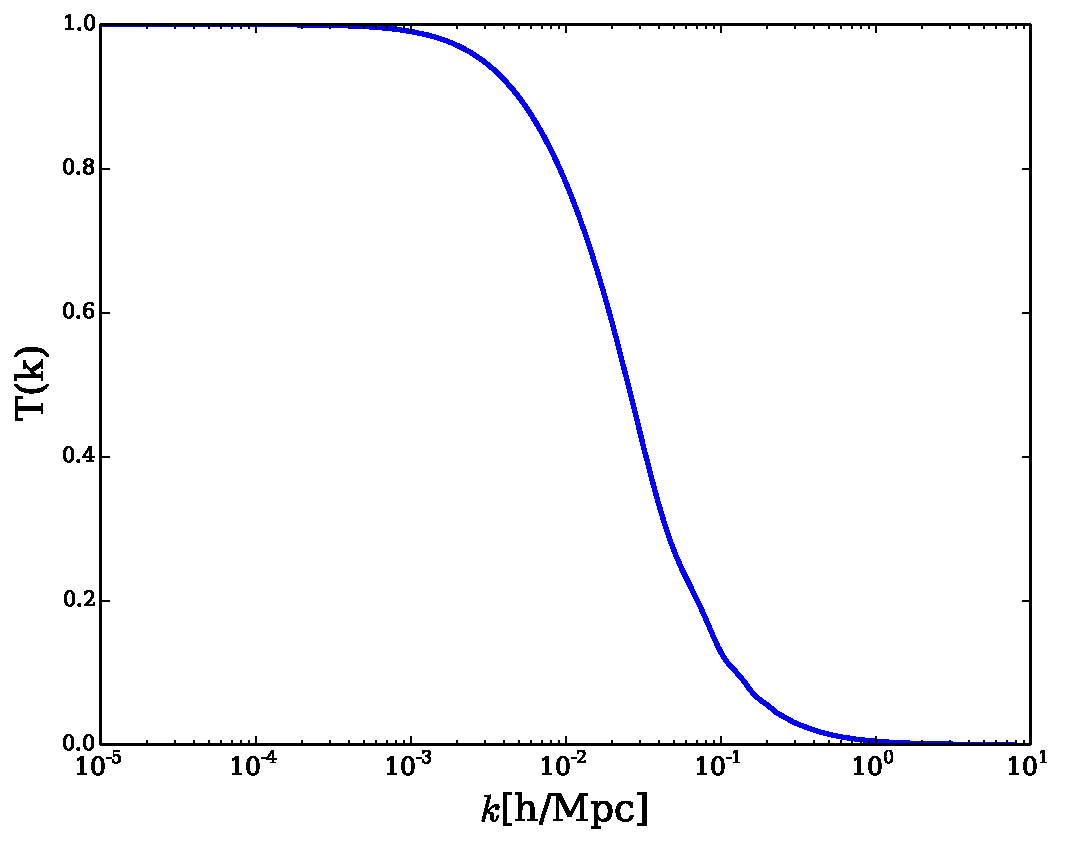
\includegraphics[width = \columnwidth]{figs/tf.pdf}
\label{tf}
\caption{Total transfer function (CDM+baryon+neutrinos) as calculated by $CAMB$.}
\end{figure}

The primordial densities grow in a complicated way as explained in the previous section; the evolved matter power spectrum can be written as redshift and wave number as
\begin{equation}
P(k,z) = P_{primordial} (k) D(z)^{2} T(k,z)^{2}
\end{equation}
where D(z) is the growth factor and T(k,z) is the transfer function. 
Growth factor for cold dark matter is given by
\begin{equation}
D(z) = H(z) \int^{\inf}_{z} \frac{dz'(1+z')}{H^{3}(z')}.
\end{equation}
The transfer function depends on the complex interactions between various components in the universe. 
While there are approximated expression for transfer function, however, the exact solution of the transfer function can only be obtained numerically. 
Numerical codes such as CAMB, CLASS etc., numerically solve the multi -component Boltzmann equations to provide T(k,z) for a given set of parameters. 

The shape of transfer function gives insight into the growth of perturbations. At early phase of the universe during radiation dominated epoch, super horizon scales grow according to the growth factor D(z) as the transfer function is unity. However, sub horizon perturbations grow only logarithmically; smaller modes entered horizon earlier than longer modes, hence had more logarithmic growth. After matter-radiation equality, perturbations grew equally on all scales. The wiggles in the transfer function at intermediate scales is due to Baryon Acoustic Oscillations (BAO). Before recombination, photons and baryons were tightly coupled, baryons experienced two opposing forces: gravitational pull due to dark matter potential well and pressure due to the radiation component resulting in oscillations of photon-baryon plasma. However, at recombination photons-baryons decouple and the baryon perturbations evolve according to the background universe. This length scale can be used as a standard ruler to measure the geometry of the universe. \pending{cite}.

~\ref{ps} shows the matter power spectrum at two different redshifts for $Planck$ 2018 cosmological parameters.The power at large scales i.e., $k<k_{eq}$ to the primordial power spectrum multiplied by the growth factor (as transfer function is unity at those scales). As one expects, the maximum of the power spectrum is directly linked to the horizon at matter-radiation equality, $k_{eq} = 0.01$.  

\begin{figure}[H]
\includegraphics[width = \columnwidth]{figs/ps.pdf}
\label{ps}
\caption{Total matter power spectrum generated by $CAMB$ for two different redshifts.}
\end{figure}